%% bare_conf.tex
%% V1.4b
%% 2015/08/26
%% by Michael Shell
%% See:
%% http://www.michaelshell.org/
%% for current contact information.
%%
%% This is a skeleton file demonstrating the use of IEEEtran.cls
%% (requires IEEEtran.cls version 1.8b or later) with an IEEE
%% conference paper.
%%
%% Support sites:
%% http://www.michaelshell.org/tex/ieeetran/
%% http://www.ctan.org/pkg/ieeetran
%% and
%% http://www.ieee.org/

%%*************************************************************************
%% Legal Notice:
%% This code is offered as-is without any warranty either expressed or
%% implied; without even the implied warranty of MERCHANTABILITY or
%% FITNESS FOR A PARTICULAR PURPOSE!
%% User assumes all risk.
%% In no event shall the IEEE or any contributor to this code be liable for
%% any damages or losses, including, but not limited to, incidental,
%% consequential, or any other damages, resulting from the use or misuse
%% of any information contained here.
%%
%% All comments are the opinions of their respective authors and are not
%% necessarily endorsed by the IEEE.
%%
%% This work is distributed under the LaTeX Project Public License (LPPL)
%% ( http://www.latex-project.org/ ) version 1.3, and may be freely used,
%% distributed and modified. A copy of the LPPL, version 1.3, is included
%% in the base LaTeX documentation of all distributions of LaTeX released
%% 2003/12/01 or later.
%% Retain all contribution notices and credits.
%% ** Modified files should be clearly indicated as such, including  **
%% ** renaming them and changing author support contact information. **
%%*************************************************************************


% *** Authors should verify (and, if needed, correct) their LaTeX system  ***
% *** with the testflow diagnostic prior to trusting their LaTeX platform ***
% *** with production work. The IEEE's font choices and paper sizes can   ***
% *** trigger bugs that do not appear when using other class files.       ***                          ***
% The testflow support page is at:
% http://www.michaelshell.org/tex/testflow/



\documentclass[conference]{IEEEtran}
% Some Computer Society conferences also require the compsoc mode option,
% but others use the standard conference format.
%
% If IEEEtran.cls has not been installed into the LaTeX system files,
% manually specify the path to it like:
% \documentclass[conference]{../sty/IEEEtran}





% Some very useful LaTeX packages include:
% (uncomment the ones you want to load)


% *** MISC UTILITY PACKAGES ***
%
%\usepackage{ifpdf}
% Heiko Oberdiek's ifpdf.sty is very useful if you need conditional
% compilation based on whether the output is pdf or dvi.
% usage:
% \ifpdf
%   % pdf code
% \else
%   % dvi code
% \fi
% The latest version of ifpdf.sty can be obtained from:
% http://www.ctan.org/pkg/ifpdf
% Also, note that IEEEtran.cls V1.7 and later provides a builtin
% \ifCLASSINFOpdf conditional that works the same way.
% When switching from latex to pdflatex and vice-versa, the compiler may
% have to be run twice to clear warning/error messages.






% *** CITATION PACKAGES ***
%
%\usepackage{cite}
% cite.sty was written by Donald Arseneau
% V1.6 and later of IEEEtran pre-defines the format of the cite.sty package
% \cite{} output to follow that of the IEEE. Loading the cite package will
% result in citation numbers being automatically sorted and properly
% "compressed/ranged". e.g., [1], [9], [2], [7], [5], [6] without using
% cite.sty will become [1], [2], [5]--[7], [9] using cite.sty. cite.sty's
% \cite will automatically add leading space, if needed. Use cite.sty's
% noadjust option (cite.sty V3.8 and later) if you want to turn this off
% such as if a citation ever needs to be enclosed in parenthesis.
% cite.sty is already installed on most LaTeX systems. Be sure and use
% version 5.0 (2009-03-20) and later if using hyperref.sty.
% The latest version can be obtained at:
% http://www.ctan.org/pkg/cite
% The documentation is contained in the cite.sty file itself.






% *** GRAPHICS RELATED PACKAGES ***
%
\ifCLASSINFOpdf
\usepackage[pdftex]{graphicx}
  % declare the path(s) where your graphic files are
\graphicspath{{./images/}}
  % and their extensions so you won't have to specify these with
  % every instance of \includegraphics
\DeclareGraphicsExtensions{.pdf,.jpeg,.png}
\else
  % or other class option (dvipsone, dvipdf, if not using dvips). graphicx
  % will default to the driver specified in the system graphics.cfg if no
  % driver is specified.
\usepackage[dvips]{graphicx}
  % declare the path(s) where your graphic files are
\graphicspath{{./eps/}}
  % and their extensions so you won't have to specify these with
  % every instance of \includegraphics
\DeclareGraphicsExtensions{.eps}
\fi
% graphicx was written by David Carlisle and Sebastian Rahtz. It is
% required if you want graphics, photos, etc. graphicx.sty is already
% installed on most LaTeX systems. The latest version and documentation
% can be obtained at:
% http://www.ctan.org/pkg/graphicx
% Another good source of documentation is "Using Imported Graphics in
% LaTeX2e" by Keith Reckdahl which can be found at:
% http://www.ctan.org/pkg/epslatex
%
% latex, and pdflatex in dvi mode, support graphics in encapsulated
% postscript (.eps) format. pdflatex in pdf mode supports graphics
% in .pdf, .jpeg, .png and .mps (metapost) formats. Users should ensure
% that all non-photo figures use a vector format (.eps, .pdf, .mps) and
% not a bitmapped formats (.jpeg, .png). The IEEE frowns on bitmapped formats
% which can result in "jaggedy"/blurry rendering of lines and letters as
% well as large increases in file sizes.
%
% You can find documentation about the pdfTeX application at:
% http://www.tug.org/applications/pdftex





% *** MATH PACKAGES ***
%
%\usepackage{amsmath}
% A popular package from the American Mathematical Society that provides
% many useful and powerful commands for dealing with mathematics.
%
% Note that the amsmath package sets \interdisplaylinepenalty to 10000
% thus preventing page breaks from occurring within multiline equations. Use:
%\interdisplaylinepenalty=2500
% after loading amsmath to restore such page breaks as IEEEtran.cls normally
% does. amsmath.sty is already installed on most LaTeX systems. The latest
% version and documentation can be obtained at:
% http://www.ctan.org/pkg/amsmath
\usepackage[braket]{qcircuit}




% *** SPECIALIZED LIST PACKAGES ***
%
%\usepackage{algorithmic}
% algorithmic.sty was written by Peter Williams and Rogerio Brito.
% This package provides an algorithmic environment fo describing algorithms.
% You can use the algorithmic environment in-text or within a figure
% environment to provide for a floating algorithm. Do NOT use the algorithm
% floating environment provided by algorithm.sty (by the same authors) or
% algorithm2e.sty (by Christophe Fiorio) as the IEEE does not use dedicated
% algorithm float types and packages that provide these will not provide
% correct IEEE style captions. The latest version and documentation of
% algorithmic.sty can be obtained at:
% http://www.ctan.org/pkg/algorithms
% Also of interest may be the (relatively newer and more customizable)
% algorithmicx.sty package by Szasz Janos:
% http://www.ctan.org/pkg/algorithmicx




% *** ALIGNMENT PACKAGES ***
%
%\usepackage{array}
% Frank Mittelbach's and David Carlisle's array.sty patches and improves
% the standard LaTeX2e array and tabular environments to provide better
% appearance and additional user controls. As the default LaTeX2e table
% generation code is lacking to the point of almost being broken with
% respect to the quality of the end results, all users are strongly
% advised to use an enhanced (at the very least that provided by array.sty)
% set of table tools. array.sty is already installed on most systems. The
% latest version and documentation can be obtained at:
% http://www.ctan.org/pkg/array


% IEEEtran contains the IEEEeqnarray family of commands that can be used to
% generate multiline equations as well as matrices, tables, etc., of high
% quality.




% *** SUBFIGURE PACKAGES ***
%\ifCLASSOPTIONcompsoc
%  \usepackage[caption=false,font=normalsize,labelfont=sf,textfont=sf]{subfig}
%\else
%  \usepackage[caption=false,font=footnotesize]{subfig}
%\fi
% subfig.sty, written by Steven Douglas Cochran, is the modern replacement
% for subfigure.sty, the latter of which is no longer maintained and is
% incompatible with some LaTeX packages including fixltx2e. However,
% subfig.sty requires and automatically loads Axel Sommerfeldt's caption.sty
% which will override IEEEtran.cls' handling of captions and this will result
% in non-IEEE style figure/table captions. To prevent this problem, be sure
% and invoke subfig.sty's "caption=false" package option (available since
% subfig.sty version 1.3, 2005/06/28) as this is will preserve IEEEtran.cls
% handling of captions.
% Note that the Computer Society format requires a larger sans serif font
% than the serif footnote size font used in traditional IEEE formatting
% and thus the need to invoke different subfig.sty package options depending
% on whether compsoc mode has been enabled.
%
% The latest version and documentation of subfig.sty can be obtained at:
% http://www.ctan.org/pkg/subfig




% *** FLOAT PACKAGES ***
%
%\usepackage{fixltx2e}
% fixltx2e, the successor to the earlier fix2col.sty, was written by
% Frank Mittelbach and David Carlisle. This package corrects a few problems
% in the LaTeX2e kernel, the most notable of which is that in current
% LaTeX2e releases, the ordering of single and double column floats is not
% guaranteed to be preserved. Thus, an unpatched LaTeX2e can allow a
% single column figure to be placed prior to an earlier double column
% figure.
% Be aware that LaTeX2e kernels dated 2015 and later have fixltx2e.sty's
% corrections already built into the system in which case a warning will
% be issued if an attempt is made to load fixltx2e.sty as it is no longer
% needed.
% The latest version and documentation can be found at:
% http://www.ctan.org/pkg/fixltx2e


%\usepackage{stfloats}
% stfloats.sty was written by Sigitas Tolusis. This package gives LaTeX2e
% the ability to do double column floats at the bottom of the page as well
% as the top. (e.g., "\begin{figure*}[!b]" is not normally possible in
% LaTeX2e). It also provides a command:
%\fnbelowfloat
% to enable the placement of footnotes below bottom floats (the standard
% LaTeX2e kernel puts them above bottom floats). This is an invasive package
% which rewrites many portions of the LaTeX2e float routines. It may not work
% with other packages that modify the LaTeX2e float routines. The latest
% version and documentation can be obtained at:
% http://www.ctan.org/pkg/stfloats
% Do not use the stfloats baselinefloat ability as the IEEE does not allow
% \baselineskip to stretch. Authors submitting work to the IEEE should note
% that the IEEE rarely uses double column equations and that authors should try
% to avoid such use. Do not be tempted to use the cuted.sty or midfloat.sty
% packages (also by Sigitas Tolusis) as the IEEE does not format its papers in
% such ways.
% Do not attempt to use stfloats with fixltx2e as they are incompatible.
% Instead, use Morten Hogholm'a dblfloatfix which combines the features
% of both fixltx2e and stfloats:
%
% \usepackage{dblfloatfix}
% The latest version can be found at:
% http://www.ctan.org/pkg/dblfloatfix




% *** PDF, URL AND HYPERLINK PACKAGES ***
%
%\usepackage{url}
% url.sty was written by Donald Arseneau. It provides better support for
% handling and breaking URLs. url.sty is already installed on most LaTeX
% systems. The latest version and documentation can be obtained at:
% http://www.ctan.org/pkg/url
% Basically, \url{my_url_here}.




% *** Do not adjust lengths that control margins, column widths, etc. ***
% *** Do not use packages that alter fonts (such as pslatex).         ***
% There should be no need to do such things with IEEEtran.cls V1.6 and later.
% (Unless specifically asked to do so by the journal or conference you plan
% to submit to, of course. )


% correct bad hyphenation here
%\hyphenation{op-tical net-works semi-conduc-tor}


\begin{document}
\newcommand{\iu}{{i\mkern1mu}}
%
% paper title
% Titles are generally capitalized except for words such as a, an, and, as,
% at, but, by, for, in, nor, of, on, or, the, to and up, which are usually
% not capitalized unless they are the first or last word of the title.
% Linebreaks \\ can be used within to get better formatting as desired.
% Do not put math or special symbols in the title.
\title{A Survey and Simulation of Three Quantum Key Distribution Protocols}

% author names and affiliations
% use a multiple column layout for up to three different
% affiliations
\author{
\IEEEauthorblockN{Conner Taylor}
\IEEEauthorblockA{cotaylor@mines.edu}}

% conference papers do not typically use \thanks and this command
% is locked out in conference mode. If really needed, such as for
% the acknowledgment of grants, issue a \IEEEoverridecommandlockouts
% after \documentclass

% for over three affiliations, or if they all won't fit within the width
% of the page, use this alternative format:
%
%\author{\IEEEauthorblockN{Michael Shell\IEEEauthorrefmark{1},
%Homer Simpson\IEEEauthorrefmark{2},
%James Kirk\IEEEauthorrefmark{3},
%Montgomery Scott\IEEEauthorrefmark{3} and
%Eldon Tyrell\IEEEauthorrefmark{4}}
%\IEEEauthorblockA{\IEEEauthorrefmark{1}School of Electrical and Computer Engineering\\
%Georgia Institute of Technology,
%Atlanta, Georgia 30332--0250\\ Email: see http://www.michaelshell.org/contact.html}
%\IEEEauthorblockA{\IEEEauthorrefmark{2}Twentieth Century Fox, Springfield, USA\\
%Email: homer@thesimpsons.com}
%\IEEEauthorblockA{\IEEEauthorrefmark{3}Starfleet Academy, San Francisco, California 96678-2391\\
%Telephone: (800) 555--1212, Fax: (888) 555--1212}
%\IEEEauthorblockA{\IEEEauthorrefmark{4}Tyrell Inc., 123 Replicant Street, Los Angeles, California 90210--4321}}




% use for special paper notices
%\IEEEspecialpapernotice{(Invited Paper)}




% make the title area
\maketitle

% As a general rule, do not put math, special symbols or citations
% in the abstract
\begin{abstract}
Private-key ciphers such as the One Time Pad are the only cryptographic systems with mathematically proven security, even against an adversary using a quantum computer. However, the One Time Pad is rarely used in practice due to the difficulty of secretly generating and distributing the long, random keys it requires. Quantum key distribution algorithms exploit the physical properties of quantum bits to provide a method for two parties to establish a shared key with guaranteed security. This paper will examine three of the most common protocols for quantum key distribution and provide a basic simulation and analysis of each.
\end{abstract}

% no keywords




% For peer review papers, you can put extra information on the cover
% page as needed:
% \ifCLASSOPTIONpeerreview
% \begin{center} \bfseries EDICS Category: 3-BBND \end{center}
% \fi
%
% For peerreview papers, this IEEEtran command inserts a page break and
% creates the second title. It will be ignored for other modes.
\IEEEpeerreviewmaketitle
\section{Introduction}
% no \IEEEPARstart
The infeasibility of large-scale key distribution for private-key cryptography has led to the widespread adoption of public-key ciphers such as RSA, which are not quantum-safe. The most secure public-key ciphers today can be broken in polynomial time by an opponent with sufficient quantum computing ability. Quantum key distribution (hence QKD) protocols attempt to improve the usability of private-key schemes such as the One Time Pad or AES by providing a secure method for generating shared keys over public channels. After the two communicating parties perform classical techniques such as error correction and privacy amplification, the key material can be used in any private-key cipher.\\

QKD protocols exploit three physical laws governing quantum bits such as polarized photons or spin-\( \frac{1}{2}\ \)particles to achieve guaranteed security:
\begin{enumerate}
\item It is impossible to duplicate an unknown quantum state without measuring it
\item Measuring a quantum bit necessarily disturbs its state
\item It is impossible to measure a quantum state in non-compatible bases simultaneously
\end{enumerate}
These properties make it impossible for an eavesdropper to gain information about a quantum key without changing it. We assume two parties, Alice and Bob, wish to establish a shared key while minimizing their mutual information with an eavesdropper, Eve. Even if Eve is allowed to intercept and modify Alice's and Bob's communication over the quantum channel, she will be unable to conceal her measurements and will be detected through classical error analysis. We assume that Eve is also capable of intercepting the classical communication between Alice and Bob, but that she is unable to alter their messages in any way. Therefore, as long as Alice and Bob use an authenticated classical channel and perform error correction and privacy amplification on their keys, Eve will be unable to gain any useful information.\\

This report will focus on three major protocols for quantum key distribution, namely the BB84 protocol proposed by Bennett and Brassard\cite{BB84}, the B92 protocol proposed by Bennett\cite{B92}, and the E91 protocol proposed by Ekert\cite{E91}. Section II will contain background material on classical cryptography and quantum bits as well as the motivation of this project. Section III will describe the three chosen protocols and compare their strengths and weaknesses. Section IV contains a description of the three simulations, their corresponding unit tests, and results. Section V will discuss the current state of QKD and an alternative six-state protocol. Solutions to selected exercises from Nielsen \& Chuang's \textit{Quantum Computation and Quantum Information} as well as the source code for the simulations will be included in the appendix.\\

\section{Background}
\subsection{Classical Cryptography}
Most electronic communications today are encrypted using a public-key cipher such as RSA\cite{Rivest}. Public-key algorithms are convenient for everyday use because, unlike private-key systems, they do not require a unique shared key for each pair of users who wish to communicate. Instead, each user possesses a private key, which is used for authentication and digital signing, and a public key, which provides confidentiality. As a result, for a system with $n$ users, any pair of whom wish to communicate, a public-key system only requires $n(n-1)$ total keys, $2n$ of which are unique. For comparison, a similar system using private-key cryptography would require $n(n-1)/2$ unique keys (see Appendix A1). For example, a system with 100 users would require 200 unique keys using RSA and 4950 unique keys using a private-key cipher.\\

However, the limitations of public-key cryptography lie in its reliance on problems which are difficult but not computationally infeasible. The most commonly used public-key cipher, RSA, relies on the difficulty of factoring composite integers\cite{Rivest}. Another type of public-key system, the elliptic curve cipher, relies on the difficulty of computing discrete logarithms\cite{Rosing}. These systems are only considered secure because no polynomial-time algorithm has been found to solve either of these problems. It has been shown that a network of computers can solve RSA classically in sub-exponential time\cite{Weisstein}, and the lower bound on time to solve these problems has not been proven. Additionally, n attacker with a sufficiently complex quantum computer can break RSA and elliptic curve ciphers in polynomial time\cite{Shor}. Although a quantum computer capable of performing Shor's algorithm on 2048-bit RSA keys is not yet practical, advances such as topological quantum computing may render public-key cryptography obsolete in the near future.\\

Unlike public-key schemes such as RSA, private-key ciphers require the generation of a new key for every pair of communicators. While this requires a much larger amount of key material, the resulting ciphertext is more secure as it does not rely on the infeasibility of solving difficult problems. Instead, the One Time Pad cipher guarantees that the ciphertext is unbreakable through either brute force or cryptanalysis. The One Time Pad is one of the simplest examples of a private-key cipher. It requires a truly random key at least as long as the message to be encrypted. To encrypt, the sender adds the key (modulo 2) bitwise with the message, and as long as the sender and recipient have the same key the recipient can perform the same operation to decrypt. This cipher is perfectly resilient to brute force attacks, since any number of valid plaintext messages can map to the same ciphertext. Unless the attacker learns the key, it is impossible to determine which plaintext is the original message. Other private-key ciphers such as Triple DES and AES use key expansion to reduce the amount of key material required while maintaining nearly perfect security.\\

In practice, private-key systems are seldom used due to limitations of classical key distribution:
\begin{itemize}
\item Keys must be truly random, as defects in pseudo-random number generators can result in low key entropy\cite{Heninger}.
\item Keys must be exchanged in secret, classically requiring a face-to-face meeting.
\item Keys must be guarded until use and destroyed afterwards.
\end{itemize}
In order for Alice and Bob to regularly exchange encrypted messages, they would have to meet in secret and generate terabytes of key material each meeting. Alternatively, they could rely on a trusted third party to generate the key material and distribute it to both of them. However, this would mean that the key is not known only to Alice and Bob, intoducing a new potential attack vector and making the key unusable for digital signing. QKD protocols address these limitations of private-key cryptography by providing a method for Alice and Bob to generate truly random, shared key material over long distances, even in the presence of eavesdroppers.\\

\subsection{Quantum Mechanics}
Part of the security of QKD arises from the fact that neither party intends to use any specific key at the outset. Instead, the key is generated truly randomly from quantum mechanical phenomena such as thermal noise\cite{Jun}. In most QKD protocols, we assume Alice begins by generating a long string of truly random classical bits. Her goal is to encode this classical information in the states of quantum bits which are subject to the physical laws discussed in Section I.\\

Quantum bits (hence 'qubits') are binary systems like classical bits, with a ``0'' state, \ket{0}, and a ``1'' state, \ket{1}. Unlike classical bits, however, a qubit can exist in a linear combination of these states called a superposition: \[ \alpha\ket{0} + \beta\ket{1}. \]According to the Measurement Postulate\cite{Kaye}, measuring a state \[ \ket{\Psi} = \sum_{i}\alpha_i\ket{\phi_i} \]with respect to the basis $B = \{\ket{\phi_i}\}$ outputs the label $i$ with probability $|\alpha_i|^2$ and leaves the system in state \ket{\phi_i}. Because measurement necessarily collapses a superposition state to one of its basis states, it is impossible for Eve to measure Alice's qubits without disturbing them and revealing her actions.\\

In quantum mechanics, measurements correspond to operators called 'observables'. The eigenvectors of an observable represent the possible measurable values of a quantum state and thus form an eigenbasis for the state space in which the observable exists\cite{Wimmel}. If two observables share at least one common eigenbasis, they are said to 'commute' and can be measured simultaneously. If they do not commute, the Heisenberg Uncertainty Principle requires that measuring one observable imparts a minimum degree of disturbance on the other\cite{Williams}. Thus, it is impossible to measure a quantum state with respect to incompatible bases simultaneously.\\

The No-Cloning Theorem states that it is impossible to clone an unknown quantum state\cite{Wootters}. To prove this, assume that there exists some unitary operator $U$ which, when applied to a quantum state \ket{\Psi}, produces a copy of the original state along with the original state. That is, \[ U\ket{\Psi}\rightarrow\ket{\Psi}\ket{\Psi}. \]The contradiction occurs when $U$ is applied to a superposition such as \[ \alpha\ket{0} + \beta\ket{1}. \]Using the linearity of unitary operators, the application of $U$ on such a superposition can be written as \[ U(\alpha\ket{0}) + U(\beta\ket{1})\rightarrow\alpha\ket{00} + \beta\ket{11}. \]However, this is not the result we expect from our definition of cloning. A cloning operator should produce the result \[(\alpha\ket{0} + \beta\ket{1})\otimes(\alpha\ket{0} + \beta\ket{1}), \]which is the original superposition state along with an exact copy of itself. Therefore, it is not possible to clone an unknown state\cite{Williams}.\\

Any two-level quantum mechanical system can be used to implement a qubit. The most common physical examples of qubits are:
\begin{itemize}
\item The energy states of electrons in an atom.
  \begin{itemize}
  \item \ket{0}, \ket{1} could be defined as ground and excited states, respectively.
  \end{itemize}
\item The magnetic spin states of spin-\( \frac{1}{2}\ \)particles such as electrons.
\item The polarization states of photons.
\end{itemize}
This paper will assume qubits are implemented as polarized photons, with the state \ket{0} representing vertical polarization and the state \ket{1} representing horizontal polarization. The possible polarization states of a photon can be visualized geometrically as three-dimensional complex vectors bounded by a unit sphere called the Bloch Sphere (see Fig. \ref{fig:blochSphere}). For example, the pure state \ket{0}, representing vertical polarization, corresponds to the unit vector in the $\hat{\textbf{z}}$ direction. Pure superposition states, where $\theta \neq \{0, \pi\}$ and $||\ket{\psi}|| = 1$, correspond to polarization axes that lie somewhere between horizontal and vertical polarization. If a photon is measured with respect to the $\{\ket{0}, \ket{1}\}$ basis, the probability it will collapse to either basis state depends on $\theta$ as well as $\phi$, the relative phase between the basis states: \[ \ket{\psi} = \cos(\frac{\theta}{2})\ket{0} + e^{\iu\phi}\sin(\frac{\theta}{2})\ket{1}. \]\\

Measuring a photon's polarization with respect to any basis is equivalent to performing a rotation operation and measuring the resulting state in the computational basis, $\{\ket{0}, \ket{1}\}$. For example, to measure the pure state \ket{0} in the Hadamard basis, $\{\frac{1}{\sqrt{2}}(\ket{0}\pm\ket{1})\}$, one can increment $\theta$ by $\frac{\pi}{2}$ to get the state \[ \ket{\psi} = \frac{1}{\sqrt{2}}(\ket{0} + \ket{1}), \] which will collapse to either the \ket{0} or the \ket{1} state with equal probibility when measured in the computational basis. The QKD protocols examined in this paper leverage the fact that the results of a measurement depend on the basis in which the measurement in performed to guarantee that any eavesdropping will be detected with high probability.\\
\begin{figure}[h]
  \hspace*{1.2cm}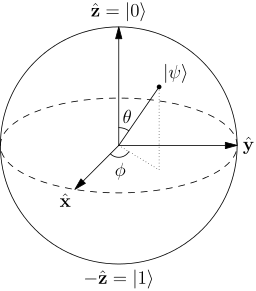
\includegraphics[width=0.4\textwidth]{bloch-sphere.png}
  \caption{The Bloch Sphere representation of a single qubit\cite{Wikipedia}.}
  \label{fig:blochSphere}
  \end{figure}

\section{Survey}
\subsection{The BB84 Protocol}
The BB84 protocol, based on Stephen Wiesner's work on conjugate coding\cite{Wiesner}, was the first QKD scheme to be proposed and is the most common QKD protocol used today. Its security relies on the fact that two non-commuting observables cannot be measured simultaneously. The protocol requires Alice and Bob to select one of two orthogonal bases at random when encoding or measuring a polarization state. These bases are the computational basis, $\{\ket{0}, \ket{1}\}$, and the Hadamard basis, $\{\ket{+}, \ket{-}\}$, where $\ket{\pm} = \frac{1}{\sqrt{2}}(\ket{0}\pm\ket{1})$. We have seen that $\{\ket{0}, \ket{1}\}$ correspond to the polarization states \ket{\uparrow} and \ket{\rightarrow}, respectively, and that $\{\ket{+}, \ket{-}\}$ correspond to the polarization states \ket{\nwarrow} and \ket{\nearrow}.\\

Although the two bases appear to be offset from each other by 45 degrees, their Bloch Sphere representation demonstrates their orthogonality. The basis states \ket{\uparrow} and \ket{\downarrow} correspond to the North and South poles of the Bloch sphere, respectively. Likewise, the \ket{\nwarrow} and \ket{\nearrow} states correspond to the East and West antipodal points in the equatorial plane\cite{Williams}.

The BB84 protocol is described as follows:
\begin{enumerate}
  \item Alice
% An example of a floating figure using the graphicx package.
% Note that \label must occur AFTER (or within) \caption.
% For figures, \caption should occur after the \includegraphics.
% Note that IEEEtran v1.7 and later has special internal code that
% is designed to preserve the operation of \label within \caption
% even when the captionsoff option is in effect. However, because
% of issues like this, it may be the safest practice to put all your
% \label just after \caption rather than within \caption{}.
%
% Reminder: the "draftcls" or "draftclsnofoot", not "draft", class
% option should be used if it is desired that the figures are to be
% displayed while in draft mode.
%
%\begin{figure}[!t]
%\centering
%\includegraphics[width=2.5in]{myfigure}
% where an .eps filename suffix will be assumed under latex,
% and a .pdf suffix will be assumed for pdflatex; or what has been declared
% via \DeclareGraphicsExtensions.
%\caption{Simulation results for the network.}
%\label{fig_sim}
%\end{figure}

% Note that the IEEE typically puts floats only at the top, even when this
% results in a large percentage of a column being occupied by floats.


% An example of a double column floating figure using two subfigures.
% (The subfig.sty package must be loaded for this to work.)
% The subfigure \label commands are set within each subfloat command,
% and the \label for the overall figure must come after \caption.
% \hfil is used as a separator to get equal spacing.
% Watch out that the combined width of all the subfigures on a
% line do not exceed the text width or a line break will occur.
%
%\begin{figure*}[!t]
%\centering
%\subfloat[Case I]{\includegraphics[width=2.5in]{box}%
%\label{fig_first_case}}
%\hfil
%\subfloat[Case II]{\includegraphics[width=2.5in]{box}%
%\label{fig_second_case}}
%\caption{Simulation results for the network.}
%\label{fig_sim}
%\end{figure*}
%
% Note that often IEEE papers with subfigures do not employ subfigure
% captions (using the optional argument to \subfloat[]), but instead will
% reference/describe all of them (a), (b), etc., within the main caption.
% Be aware that for subfig.sty to generate the (a), (b), etc., subfigure
% labels, the optional argument to \subfloat must be present. If a
% subcaption is not desired, just leave its contents blank,
% e.g., \subfloat[].


% An example of a floating table. Note that, for IEEE style tables, the
% \caption command should come BEFORE the table and, given that table
% captions serve much like titles, are usually capitalized except for words
% such as a, an, and, as, at, but, by, for, in, nor, of, on, or, the, to
% and up, which are usually not capitalized unless they are the first or
% last word of the caption. Table text will default to \footnotesize as
% the IEEE normally uses this smaller font for tables.
% The \label must come after \caption as always.
%
%\begin{table}[!t]
%% increase table row spacing, adjust to taste
%\renewcommand{\arraystretch}{1.3}
% if using array.sty, it might be a good idea to tweak the value of
% \extrarowheight as needed to properly center the text within the cells
%\caption{An Example of a Table}
%\label{table_example}
%\centering
%% Some packages, such as MDW tools, offer better commands for making tables
%% than the plain LaTeX2e tabular which is used here.
%\begin{tabular}{|c||c|}
%\hline
%One & Two\\
%\hline
%Three & Four\\
%\hline
%\end{tabular}
%\end{table}


% Note that the IEEE does not put floats in the very first column
% - or typically anywhere on the first page for that matter. Also,
% in-text middle ("here") positioning is typically not used, but it
% is allowed and encouraged for Computer Society conferences (but
% not Computer Society journals). Most IEEE journals/conferences use
% top floats exclusively.
% Note that, LaTeX2e, unlike IEEE journals/conferences, places
% footnotes above bottom floats. This can be corrected via the
% \fnbelowfloat command of the stfloats package.

\section{Conclusion}
Classical private-key encryption systems are only secure as long as the keys used are exchanged in advance, protected until they are needed, and then destroyed. These limitations are the reason why the key distribution problem is one of the biggest drawbacks of private-key cryptosystems. Quantum Key Distribution protocols provide a possible solution to this problem by exploiting the physical properties of small particles, which comprise the 'qubits' of a quantum computer.\\

Because the quantum state represented by a qubit cannot be observed or copied without disturbing the state, an eavesdropper cannot intercept a key transmitted through a quantum channel without modifying the keystring. By performing a survey of several implementations of quantum key distribution protocols, we will attempt to determine the security advantages and disadvantages QKD offers compared to classical key distribution techniques.\\

% conference papers do not normally have an appendix
% use section* for acknowledgment

% trigger a \newpage just before the given reference
% number - used to balance the columns on the last page
% adjust value as needed - may need to be readjusted if
% the document is modified later
%\IEEEtriggeratref{8}
% The "triggered" command can be changed if desired:
%\IEEEtriggercmd{\enlargethispage{-5in}}

% references section
% can use a bibliography generated by BibTeX as a .bbl file
% BibTeX documentation can be easily obtained at:
% http://mirror.ctan.org/biblio/bibtex/contrib/doc/
% The IEEEtran BibTeX style support page is at:
% http://www.michaelshell.org/tex/ieeetran/bibtex/
%\bibliographystyle{IEEEtran}
% argument is your BibTeX string definitions and bibliography database(s)
%\bibliography{IEgEEabrv,../bib/paper}
%
% <OR> manually copy in the resultant .bbl file
% set second argument of \begin to the number of references
% (used to reserve space for the reference number labels box)

\begin{thebibliography}{15}
\bibitem[1]{BB84}
  C. H. Bennett and G. Brassard, ``Quantum Cryptography: Public Key Distribution and Coin Tossing,'' Intl. Conf. on Computers, Systems, \& Signal Processing, 12 Dec. 1984.
\bibitem[2]{B92}
  C. H. Bennett, ``Quantum Cryptography Using Any Two Nonorthogonal States,'' Phys. Rev. Lett., Volume 68, Number 21, 25 May 1992.
\bibitem[3]{E91}
  A. K. Ekert, ``Quantum Cryptography Based on Bell's Theorem,'' Phys. Rev. Lett., Volume 67, Number 6, 5 August 1991.
\bibitem[4]{Rivest}
  R. Rivest, A. Shamir, and L. Adleman, ``On Digital Signatures and Public Key Cryptosystems,'' Commun. Ass. Comp. Mach., Volume 21 (1978) pp. 120-126.
\bibitem[5]{Rosing}
  M Rosing, ``Implementing Elliptic Curve Cryptography,'' Manning Publications, Greenwich (1999) ISBN 1-884777-69-4.
\bibitem[6]{Weisstein}
  E. W. Weisstein, ``RSA-640 Factored,'' MathWorld Headline News, 8th November (2005),
  http://mathworld.wolfram.com/news/2005-11-08/rsa-640/.
\bibitem[7]{Shor}
  P. Shor, ``Polynomial-time Algorithms for Prime Factorization and Discrete Logarithms on a Quantum Computer,'' Siam Journal on Computing, Volume 26, Issue 5 (1997) pp. 1484-1509.
\bibitem[8]{Heninger}
  N. Heninger, Z. Durumeric, E. Wustrow, J. A. Halderman, ``Mining Your Ps and Qs: Detection of Widespread Weak Keys in Network Devices,'' Proc. 21st USENIX Security Symposium, Aug. 2012.
\bibitem[9]{Jun}
  B. Jun and P. Kocher, ``The Intel Random Number Generator,'' Cryptography Research, Inc. white paper prepared for Intel Corp., 22 Apr. 1999.
\bibitem[10]{Kaye}
  P. Kaye, R. LaFlamme, M. Mosca, \textit{An Introduction to Quantum Computing}, Oxford UP, 2010. Print. ISBN 978-0-19-857049-3.
\bibitem[11]{Wimmel}
  H. Wimmel, \textit{Quantum Physics \& Observed Reality: A Critical Interpretation of Quantum Mechanics}, World Scientific, 1992. Print. ISBN 981-02-1010-8.
\bibitem[12]{Williams}
  C. Williams, \textit{Explorations in Quantum Computing}, Springer, 2011. Print. ISBN 978-1-84628-886-9.
\bibitem[13]{Wootters}
  W. K. Wootters and W. H. Zurek, ``A Single Quantum Cannot Be Cloned,'' Nature, Volume 299, pp. 802-803. 28 Oct. 1982.
\bibitem[14]{Wikipedia}
  Wikipedia, the free encyclopedia, ``Bloch Sphere,''
  URL: https://upload.wikimedia.org/wikipedia/commons/thumb/f/f4/Bloch\_Sphere.svg/256px-Bloch\_Sphere.svg.png
\bibitem[15]{Nielsen}
  M. Nielsen and I. Chuang, ``Quantum Computation and Quantum Information,'' Cambridge UP, 2015. Print.
\end{thebibliography}




% that's all folks
\end{document}
